
In this section, we consider a communication-theoretic meaning of the optimization problem \eqref{eqmainproblem}. Consider a feedback control architecture shown in Figure~\ref{fig:NCS}. 


\begin{figure}
\centering
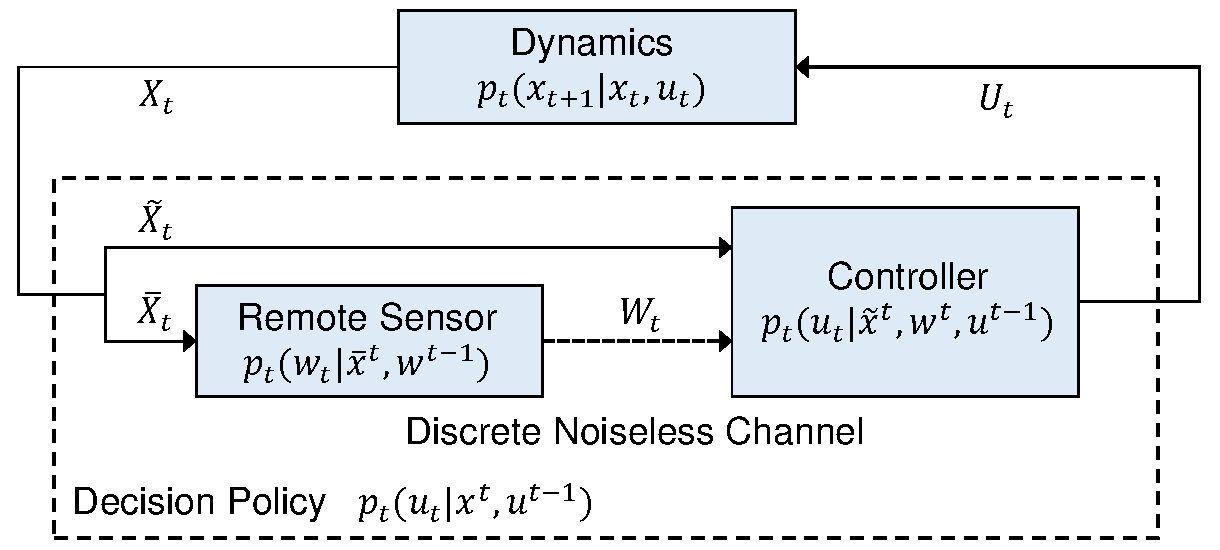
\includegraphics[width=\columnwidth]{comm.pdf}
\caption{Example of a feedback control structure with remote and local sensors}
\label{fig:NCS}
\end{figure}


At every time step $t$, assume that the free component $\tilde{X}_t$ of the state vector is immediately available to the controller, while the expensive component $\bar{X}_t$ is only available at a remote sensor. The remote sensor produces a discrete codeword $W_t\in\mathcal{W}_t$ based on a policy $p_t(w_t|\bar{x}^t, w^{t-1})$, where $\mathcal{W}_t$ is a certain codebook such that $|\mathcal{W}_t|=2^{R_t}$. Codeword is transmitted over a noiseless communication channel and received by the controller without delay, and a control input $U_t$ is generated based on a policy $p_t(u_t|\tilde{x}^t, w^t, u^{t-1})$.
Assuming that transmitting data over the communication channel incurs unit cost $\beta$ per \emph{bit}, consider the following communication design problem
\begin{equation}
\min_{\{\mathcal{W}_t, p_t(w_t|\bar{x}^t, w^{t-1}), p_t(u_t|\tilde{x}^t, w^t, u^{t-1}) \}_{t=0}^{T-1}}  J(X^T, U^{T-1}) +\beta R \label{eqcommproblem}
\end{equation}
where $R=\sum_{t=0}^{T-1}R_t$ is the total amount of data. 
The next result shows that \eqref{eqdi} provides a lower bound to $R$.
\begin{theorem}
\label{theorate}
Suppose that the plant dynamics is given by an MDP $M$. For any choice of the codebook $\mathcal{W}_t$, sensor policy $p_t(w_t|\bar{x}^t, w^{t-1})$ and controller policy $p_t(u_t|\tilde{x}^t, w^t, u^{t-1})$ for $0\leq t\leq T-1$ in Figure~\ref{fig:NCS}, we have
\[
R \geq I(\bar{X}^{T-1}\rightarrow U^{T-1}\| \tilde{X}^{T-1}).
\]
\end{theorem}
\begin{proof}
See Appendix \ref{sec:prf}
\end{proof}
Theorem~\ref{theorate} shows that the optimization problem \eqref{eqmainproblem} provides a fundamental performance limitation of the networked control system shown in Figure~\ref{fig:NCS} in that the optimal value of \eqref{eqcommproblem} is lower bounded by the optimal value of \eqref{eqmainproblem}.




%Consider Figure \ref{fig:NCS}. Assume that transmitting data for $\bar{X}$ over the communication channel incurs unit cost $\beta$ per \emph{bit}, and now consider the following communication design problem
%\begin{equation}
%\min_{\{\mathcal{W}_t, p_t(w_t|\bar{x}^t, w^{t-1}), p_t(u_t|\tilde{x}^t, w^t, u^{t-1}) \}_{t=0}^{T-1}}  J(X^T, U^{T-1}) +\beta R \label{eqcommproblem}
%\end{equation}
%where $R=\sum_{t=0}^{T-1}R_t$ is the total amount of data. 
%The next result shows that \eqref{eqdi} provides a lower bound to $R$.
%\begin{theorem}
%	Suppose that the plant dynamics is given by an MDP $M$. For any choice of the codebook $\mathcal{W}_t$, sensor policy $p_t(w_t|\bar{x}^t, w^{t-1})$ and controller policy $q_t(u_t|\tilde{x}^t, w^t, u^{t-1})$ for $0\leq t\leq T-1$ in Figure \ref{fig:NCS}, we have
%	\[
%	R \geq I(\bar{X}^{T-1}\rightarrow U^{T-1}\| \tilde{X}^{T-1}).
%	\]
%\end{theorem}
%\begin{proof}
%	Appendix.
%\end{proof}

%In this section we present a physical intepretation of the use of transfer entropy in this problem formulation in the case of a networked control problem. We will prove the rate of communication $R(D)$ will be lower bounded by the directed information. We first prove the following lemma.
%\begin{lemma}
%\begin{align}
%I(X_1^T \rightarrow U^T || X_2^T) \leq I(X_1^T \rightarrow W^T || U^{T-1},X_2^T)
%\end{align}
%\end{lemma}
%\begin{proof}
%\begin{align*}
%0 &\leq I(X_1^T \rightarrow U^T || X_2^T) - I(X_1^T \rightarrow W^T || U^{T-1},X_2^T) \\
%& = \sum_{t=1}^T I\left(X_1^t;W_t|W^{t-1},U^{t-1},X_2^t \right) - I\left(X_1^t;U_t|U^{t-1},X_2^t \right)\\
%& = \sum_{t=1}^T I\left(X_1^t;W_t,U_t|W^{t-1},U^{t-1},X_2^t \right) \\&- I\left(X_1^t;U_t|U^{t-1},X_2^t \right)\\
%& = \sum_{t=1}^T I\left(X_1^t;W_t|U^{t},X_2^t \right) - I\left(X_1^t;W^{t-1}|U^{t-1},X_2^t \right)\\
%& = \sum_{t=1}^T I\left(X_1^t;W_t|U^{t},X_2^t \right) - I\left(X_1^{t-1};W^{t-1}|U^{t-1},X_2^{t-1} \right)\\
%& = I\left(X_2^T;W^T | U^T,X_1^T \right) \geq 0 
%\end{align*}
%\end{proof}
%The third line follows from the fact 
%\begin{align*}
% I & \left(X_1^t;W_t,U_t| W^{t-1},U^{t-1}, X_2^t \right) =  \\ & I\left(X_1^t;W_t|W^{t-1},U^{t-1},X_2^t \right) + I\left(X_1^t;U_t|W^{t},U^{t-1},X_2^t \right) = \\ & I\left(X_1^t;W_t|W^{t-1},U^{t-1},X_2^t \right)
%\end{align*}
%The next line follows from using the chain rule. 
%
%We now present one of the main results of the paper. 
%\begin{theorem}
%$R(D) \geq I(X_1^T \rightarrow U^T || X_2^T)$
%\end{theorem}
%
%\begin{proof}
%\begin{align*}
%\sum_{t=1}^T R_t &\geq \sum_{t=1}^T H(W_t)\\
%&\geq \sum_{t=1}^T H(W_t\vert W^{t-1},U^{t-1},X_2^t)\\
%&\geq \sum_{t=1}^T H(W_t\vert W^{t-1},U^{t-1},X_2^t) - H(W_t\vert X_1^t, W^{t-1},U^{t-1},X_2^t)\\
%& =  \sum_{t=1}^T I \left(X_2^T \rightarrow W^T \vert \vert U^{T-1},X_2^{T} \right)\\
%& \geq I \left(X_1^T \rightarrow U^T \vert \vert X_2^T \right)
%\end{align*}
%\end{proof}